\documentclass{article}
\usepackage{a4}
\usepackage{graphicx}
\usepackage{algorithm}
\begin{document}
\title{The Engine Behind Model Checking}
\maketitle
\begin{center}
\textbf{Reema Patne \\ Swansea University \\ Under the guidance of Dr. Oliver Kullmann }
\end{center}
\begin{abstract}
In order to ensure the safety and quality of a system, it is necessary to undergo a process of system validation which checks the correctness of specifications, designs and products. The various validation techniques are peer reviewing, simulation, formal verification, and model checking, etc. Of all the techniques, model checking has become the most popular approach in the both hardware and software areas due to the availability of various support tools and its success in the project. This project is all about understanding the engine behind model-checking. SAT-Technology is emerging as a central engine used in model checking tools. The principle behind it is very simple: formulate everything at the (logical) gate-level, and then run a SAT solver. The devil is then in the details. This project is about exploring this fascinating and recent connection. Either gaining some overview, or exploring a concrete application. The model, the logical side of it, the SAT side of it is a planned task for the document to write. This report has been written as the results of the literature survey and the specification.
\end{abstract}

\newpage
\tableofcontents
\maketitle
\newpage

\section{Introduction}
\label{sec:intro}
Describing what a system is required to do is known as system specification. By doing so, we will be able to understand the system. Various validation techniques are used to check the correctness of specification. It guarantees the quality of the system and also its safety [8]. Model checking is one of the most popular validation techniques. For a system defined in finite state model and a property defined in terms of logical formalism, model checking techniques could systematically check the validity of this property [15]. A finite-state model is used to design computer programs and digital logic circuits. It is as an abstract machine that can be in one of a finite number of states. It will be only in one state at a time; the state it is in at any given time is called the current state. When initiated by a triggering event or condition, the state changes, this is called a transition. 
Roughly, M is an abstract model of a system whose structure is defined as finite-automata and $\phi$  is a logical formula specifying a desirable property such that M satisfies $\phi$  abbreviated as $M \models \phi$. 
Model checking helps from preventing the bugs even before penning down the code of the project i.e., during the requirement and the design phase itself. It prevents the further breed of the bugs and hence it makes sense by being cost effective [7]. The errors which are not been able to find by simulation is done by model checking by considering all possible behaviours of the system[3]. 
Model checking is the one of the foremost applications of logics which ranges from computer science to computer engineering. Since then, there has been a multiple breakthrough. The gap which was built between the theoretical computer science, hardware and software engineering was bridged by Model Checking. Now, model checking has been extensively used for verifying many Software and also used in hardware industry. It has virtually became a universal tool for the analysis of the systems. Henceforth, this project will focus on the state of the art of model checking.

\section{Literature Survey}

\subsection{Model Checking}
\label{Model Check}
The technique used for validating a system is Model checking. The design process and the validation process are the must to ensure the correctness of specifications, designs and products of the system. Validation is done to see that whether the system meets all its requirements. The two types of validation techniques are: 
\begin{itemize}
\item Informal ones which include peer testing and testing.	
\item Formal ones which include formal verification, simulation and model checking. 
\end{itemize}	
This report focuses on the Formal validation technique – Model Checking. Model checking systematically checks the validity of a given finite-state model of a system and properties stated in the form of logical formalism such as temporal logic. It uses algorithms which are executed by the computer tools. The inputs to such model checkers are the description of the model and the description of the properties. Once these files are fed as an input, the model checker performs the verification. If error occurs, then the model checker provides the counter-example to explain under which circumstances the error can be generated. This counter-example helps in finding the error and repairing the specifications of the model. This can be shown with help of the following diagram. It shows us how the verification process takes place in the model checking.  
\subsubsection{Systems and their Specifications}
\label{Sys Spec}
Describing a system is called specification. Specification helps in finding errors and    understanding a system. So, it is a good practise to have a clear idea about the design and improve it before the implementation. The specification of the system can be functional or non-functional i.e. what a system is supposed to do or performance properties. These specifications are written in formal language with proper syntax and semantics which can be verified and validated with respect to requirements. 
It helps in developing the explicit model of a system which is clear, precise and unambiguous. Mathematics is used as a basic tool to achieve this. Here, reading the accompanying words in order to understand the relation between the equations is a bit tedious. In order to overcome this shortcoming using mathematics as a basic tool, logicians have temporal logic which is precise and completely formal mathematics. This temporal logic is used in such a way so as to describe the system behaviour.  
\subsubsection{Temporal Logic}
\label{Temp Logic}
There are various interpretations of temporal logic depends on the individual as how to consider the system with time. It is the logic for expressing mathematics. It supports formulating the properties of the system behaviour with respect to time. There are various types of temporal logics:
\begin{itemize}
\item •	Temporal Logics used to specify the reactive systems are: \\
\textbf{Linear temporal logic:}It allows the statement of properties of execution sequences of a system. \\
 \textbf{Branching temporal logic:}It allows the user to write formulas which include some sensitivity to the choices available to a system during its execution.
\end{itemize}
These two kinds of temporal logic are characterized by a continuous interaction with the environment [15].
\begin{itemize}
\item •	Temporal Logics used to specify the time-critical systems:\\
 \textbf{Real-Time temporal logic:}  It allows statement of properties of multiple concurrent processes and supports relative time references.
\end{itemize}
It is characterized by quantitative timing properties relating occurrences of events [15].
In order to avoid the errors we write specifications. Validation techniques are used to checking the correctness of the system.  
\subsubsection{Model-Checking Algorithm}
\label{Model chec Algo}
Model checking uses exhaustive state space search of the system model as 	algorithm: The desired properties satisfied for each state of the model. 	Reachability property is used to check whether the system can reach a state without any deadlocks. Reachability is considered as one of the important property which uses Reachability analysis technique. It starts from initial system state and see to it that it reaches all the possible system states which can be reached. For instance, in a traffic signal model, yellow, red and green are the three states. Model checking proves if it can reach some state, all the states are eventually got by the model, or if the model could never get some state.
\subsubsection{Approaches Of Model Checking}
\label{Appr to model check}
\begin{itemize}
\item Logic based approach: Here the system is modelled as finite-state automaton representing the states as values of variables and control location, and changes of a system from one state to other state is represented by transition. If a system satisfying the desired behaviour given in some logic with the initial set of states, then the system is said to be correct.
\item Behaviour based approach: Given the desired and the possible behaviour with the same notation, the equivalence relations are used as criteria for the correctness. Hence, if the desired and the possible state behaviour are equivalent then the system is said to be correct.  
\end{itemize}
\subsubsection{Model Checkers}
In verifying a system, model checking techniques uses tools known as model checkers. Due to the progress of model checking, industries are developing their own model checkers. 
Exhaustible list of  Model Checkers are given below:
\begin{description}
\item[Blast model checker:]Berkeley Lazy Abstraction Software Verification Tool abbreviated as BLAST .It is a model checking tool used for C programs.
\item[CADP:]Commonly known as  Construction and Analysis of Distributed Processes.It uses the formal description technique and software tools for simulation to facilitate the design of reliable systems.
\item[Chess model Checker:]It is a software which uses thread schedules to find bugs or errors in multi-threaded software such as deadlocks,data-corruption which are hard to find using testing tools.It helps in debugging the process by providing the full repeatable execution of the program which is causing an error.
\item[CHIC:] Commonly known as Checker for Interface Compatibility. It is used in hardware and software systems to verify the behavioural compatibility.
\item[FDR:] Commonly called as Failures-Divergences Refinement is the software tool used to check  the refinement.
\item[ISP:] Commonly known as In-situ Partial Order .It is a formal verification tool.They perform the verification at the level of code.It has successfully verified the codes for deadlocks and assertion violations.
\item[Java pathfinder:]The executable Java byte-code programs are verified by this Java pathfinder system.It does the model checking for the concurrent programs.As using this it helps in detecting the deadlocks and data races.It can also be used to model check the distributed applications and user interfaces.
\item[LTSA:] It is commonly known as Labelled Transition System Analyser. It is used to verify the concurrent systems. FPS process algebra is used to describe LTSA. The systems are finite state machines.
\item[MRMC:] Commonly known as Markov Reward Model Checker is tool written in C programming language.It model checks for discrete-time models and continuous –time model.Within a given time and within the constraint it checks the reachability of the set of goal states.
\item[mCRL2 Toolset:]It is used to describe the concurrent systems since it uses the specification language.
\item[MoonWalker:]It model checks for .Net applications by detecting the errors.Also it is able to find the deadlocks and assertion violations as well.
\item[NuSMV:] It is the expansion of  symbolic model checker.It provides verification for industrial designs.Also it provides analysis of specifications.
\item[Ompca:]It is commonly known as Open MP C Analyser .It helps in model checking  real-time systems with dense-time models.It is an application for timed automata’s.
\item[PAT:]It is commonly known as process analysis tool kit.It helps concurrent and real-time systems in reasoning and simulating.It helps in solving deadlocks and reachability.
\item[PRISM:]It is commonly called as probabilistic model checker.It is used in model checking for the system that exhibits probabilistic behaviour.This software tool is used in modelling and analysis of the system.
\item[Rabbit:]It does model checking by providing the reachability analysis and refinement.It is used for real-time systems.
\item[REDLIB:] It is a model checker for timed automata’s.It helps in verification tasks.
\item[SMART:] It is a model checker used to check the reliability and timing.
\item[Spin Model Checker:]It verifies the correctness of the models in automated fashion. This is one of the biggest achievements. It avoids pre-construction of the states.
\item[TAPA’s:]It is a tool used in concurrent systems for specifying and analysing.It also helps in model checking temporal formulas.
\item[Vereofy:]This model checker checks for operational correctness .It model checks for component-based systems.
\item[mCRL:] It studies description and analysis of distributed systems.It solves the problem in a very simple manner using the algebras CCS,CSP and ACP.
\item[UPPAAL:]It is used for real-time systems for modelling,validation and verification.
\item[Romeo:]This is same as UPPAAL which is used for modelling,validation and verification of the real-time systems.
\item[TLA+:]It is commonly called as Temporal Logic Of Actions.It combines logic of actions with temporal logic.In concurrent systems TLA+ is used in describing its behaviour.
\item[AlPina:]It is commonly called as Algebraic Petri Nets Analyser.It provides model checking for algebraic petri nets.
\item[McErlang:]It is a model checker used in checking the programs written in erlang language.
\end{description}
\subsection{Technology}
\label{tech}
Model checking then, used explicit state traversal where the reachable state space was traversed to find the errors violating the safety properties. It consumed lot of space in the computer memory because each state of the system was stored in large hash table. In order to improve this space consumption in explicit state model checker various techniques came into existence. SPIN model checker was the most successful explicit model checker. The goal of this was to overcome the state explosion problem where the states of the model were represented symbolically. 
Later in mid-80's Binary Decision Diagrams as a new data structure came into existence for symbolical representation and manipulating Boolean functions efficiently [4] known as Symbolic model checking with BDDs. BDDs could handle much larger designs with hundreds of state variables representing Boolean functions. There existed some shortcoming in BDDs as well. They became too large to handle as they used canonical representation. BDDs required uniform variable ordering along the paths and it sometimes happened that no space efficient variable ordering existed. This was time consuming and needed manual intervention. 
There came into existence the SAT procedures as an alternative approach to model checking. Unlike BDDs, it didn’t use the canonical representation. It became one of the most efficient implementation. It overcame the state explosion problem faced by BDDs. 
In late 90s, researchers came up with the idea of Bounded model checking which uses SAT solvers to the model checking problem. Bounded model checking technique do a fast exploration of state space overcoming the shortcomings of the previous approaches using the SAT procedures instead of BDDs where the SAT has a depth first search nature. This method is applicable for properties which include safety and liveness where it checks whether a given set of states is reachable, and detects loops in a system’s state transition graph.
\subsection{Example to illustrate the new technique}
\label{Example}
Application of Model Checking ranges from simple coffee machines to nuclear plants which are undoubtedly critical and the failure of which may cause economical and physical damages. Considering an example of a coffee machine, where the system is fed with a sensitive data to check the behaviour of the system as it is supposed to behave. This is known as testing. 
 \begin{figure}[h!]
 \centering
 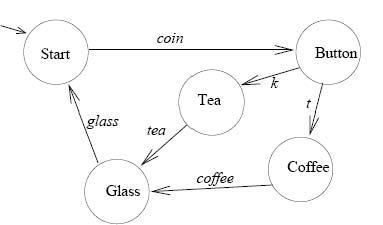
\includegraphics[width=0.5\textwidth]{flower.png}
\caption{Finite states of a coffee machine.}
 \end{figure}
 A coffee machine consists of a set the following above states which are depicted in circles and relations as arrows between the states. Arrows are given with labels representing actions. The combination of this set of states and relations is known as ``automaton".  If the given action on an arrow connecting both the states is satisfied, then automaton in a given state changes to another state. 
Initially the machine is at state ``Start" and it ``waits" for a coin. If a coin is provided then the machine change state to the ``Button" state where two options are possible: to press the ``k" button and then go to the ``Coffee" state, or to press ``t" and go to the ``Tea" state. After serving the corresponding drink, the machine goes to the "Glass" state and it gives a glass with the chosen drink to then go back to the ``Start" state.
\paragraph{Example 1}
The property ``Always, after the machine gets a coin and the user press a button, it gives coffee or tea", can be written in temporal logic as:
ALWAYS (IF Button THEN (SOMETIME-IN-THE-FUTURE (Coffee OR Tea)))
Words in upper-case are temporal logic ``connectives" or ``operators", and the other words represent the interaction between the machine and the user. The above expression is a ``formula" of temporal logic.
How can one see that the given automaton satisfies a formula? We can explain it by using the above formula and the automaton modelling the coffee machine.
Let us assume the current state of the automaton is the initial ``Start" state. Let A and B be statements, then ``ALWAYS A" means that A must be true in all the states of the automaton. ``IF A THEN B" means that whenever A is true in a given state, so is B. ``A OR B" means that at least one of A and B must be true in the state. Finally ``SOMETIME-IN-THE-FUTURE A" means that it must exist a state in the future of the current state where A is true.
It is then possible to check that the above formula is satisfied by the automaton, since from the state ``Button" (after a coin is inserted) it is possible to find a state in the future such that the actions ``coffee" or ``tea" are possible.
\paragraph{Example 2}
Let us consider now the following property: ``Always, after pressing a button the machine will serve coffee and then tea immediately afterwards". We can write this sentence as follows:
ALWAYS (IF Button THEN (Coffee AND NEXT Tea))
Here NEXT is a connective formalising the ``immediately after" English expression. As for the previous example it is possible to check whether the automaton satisfies the property. In this case we can see that it is not the case, since from the state ``Button" one can reach the state ``Coffee" and ``Tea", but from the ``Coffee" state it is not possible to go immediately after to the ``Tea" state. This property guarantees that the machine will never allow to get coffee and then tea by paying only once.
\section{Making the Specifications Executable}
It is difficult to validate the system with the specifications and requirements. The     validation task would be easier if we make the specifications executable, giving the immediate feedback of the behaviour of the future software to the user.
	The boolean level of representation of the model-checking task with the   computation engine that supported the required set of operations gave  rise to Symbolic model checking. Ordered Binary Decision Diagram(OBDD) was the first approach combining the efficiency and expressive power. Recently, based on Davis-Putnam-Logemann-Loveland (DPLL) algorithm, Boolean satisfiability(SAT) checkers have greatly extended the reach of bounded model checkers.
OBDDs and DPLL –based checkers compliments each other. OBBDs readily deal with quantified Boolean formulas(QBF) where as DPLL cannot. SAT problem which are completely intractable for DPLL are trivial with OBDDs. SAT checkers are insensitive to the number of variables. 
\subsection{A view from the engine room}
The first symbolic model checkers used Ordered Binary Decision Diagrams (OBDDs) [5] to represent system transition relations and sets of system states [2]. All the steps required for a model checking is expressed as a series of operations on these representations, without enumerating individual states or transitions. Recently, Bounded and In bounded model checking has been devised which use Boolean satisfiability (SAT) solvers as a computational engines. Combining the methods which have a SAT solver work on a detailed system model and OBDDs operate on a abstracted model, is more powerful than operating on its own[8].
Model checkers are now able to handle the complex verification problems coming from real world hardware and software designs with the help of Boolean methods. By giving the importance of Symbolic model checking, I take this opportunity to examine the capabilities of SAT solver.
\subsection{Experiments in (Un)SAT:}
When the given task is to prove that the given formula is unsatisfiable, we find an error in the design by using the SAT solver which is typically used by verification problem. To prove that the formula is unsatisfiable, it is currently highly favourable to use DPPL method [13].for solving SAT problems by backtracking search among complete SAT algorithms. By doing so, it has gained a remarkable progress in speed and capacity[14].
I would be working on the SAT Solver Performance in Solving Associativity Problems 
Considering a class of benchmarks, we consider ones that model the bit-level behavior of arithmetic operations. Consider the problem of proving that integer addition and multiplication are associative. That is, we wish to show that the following two C functions always return the value 1:
\begin{algorithm}
int assocA(int x, int y, int z)\\
\{\\
return (x+y)+z == x+(y+z);\\
\}\\
int assocM(int x, int y, int z)\\
\{\\
return (x*y)*z == x*(y*z);\\
\\
\}
\end{algorithm}

We created a set of benchmark problems from these C functions, where we varied the number of bits n in the argument words x, y, and z, up to a maximum of n=32. Since there are three arguments, the number of possible argument combinations is $8^{n}.\\
Numbers indicate the maximum word size that can be solved in under $900 seconds of CPU time.
\begin{table}[htb]
\centering
\begin{tabular}{|c|c|c|c|}
\hline
Problem & Exhaustive & CUDD & MINNISAT \\ [0.5ex]
\hline
Addition & 12 & \textgreater 32 & \textgreater 32\\
Multiplication & 12 & 8 & 5\\
\hline

\end{tabular}
\end{table}



In each case, we show the maximum number of argument bits n for which the problem can be solved within a 900 second time limit. Exhaustive evaluation works up to n = 12, but then becomes impractical, with each additional bit requiring eight times more evaluations. Both DPLL and OBDDs can show that addition is associative up to the maximum value tested. For multiplication, we see that OBDDs outperform DPLL, but neither does as well as brute-force, exhaustive evaluation. For OBDDs, we know that the Boolean functions for integer multiplication require OBDDs of exponential size [6], and hence OBDD-based methods for this problem incur exponential space and time. Evidently, DPLL-based methods also suffer from exponential time performance.
\section{Observation}
\label{observe}
Our arithmetic problems illustrate that, while both DPLL and OBDDs are adequate for addition and related functions, neither performs well for operations related to integer multiplication. Indeed, companies that market circuit equivalence checkers have had to devise ad hoc workarounds for checking circuits containing multipliers. We believe that the research community should invest more effort in tackling problems that are well beyond the capability of existing SAT solvers. Examples of challenging problems arise in the fields of cryptanalysis [11] and combinatorial optimization.
\section{Project Schedule}
\label{Project Schd}

This section will give an overview of how this project will be constructed and how to manage this project.
\begin{itemize}
\item Since the model checking being a very exhaustive field and also theoretical, I would take approximately around one month i.e., june to concentrate on the basics of  model checking. I would be going thoroughly into the books called “ Systems ans Software Verification ” by B.Berard for understanding the Model-Checking Techniques and Tools, “ Software Abstractions ” by Daniel Jackson for understanding the Logic, Language ans Analysis, “ Tuning SAT-Checkers for Bounded Model-Checking ” and “ Heuristics for Efficient SAT solving ” by Strichman.
\item  By gaining the thorough knowledge about the model checking and understanding its basics, the next two months i.e., in the month of july and august I will be learning how the Model checking software works. I will be going through the various websites to understand the software.
\item And in the month of september I will be in a position to give my own example and check how it works.
\end{itemize}
\section{Challenges Facing}
\begin{itemize}
\item Learning the usage of Github: It is a website used for storing and presenting our files. Git is a decentralized version control system that is used by a number of open source projects, most notably perhaps the Linux kernel. GitHub is a new hosted Git repository service that's being called a "social network" for programmers and with good reason. In my project it helps in communication between me and my supervisor by providing information to assist in evaluating the tools and making an informed decision.
\item Learning the usage of LATEX: It is a document preparation system similar to that of a Microsoft word where the similarities end here. Preparing a document with LATEX consists of using a text editor to edit a Latex source file with the .tex extension. And then running a latex program to convert the source file to a document interchange format like PDF etc. Doing in LATEX provides a good typography which provides a good impression on the content of the document and is platform independent unlike MS word which runs only on windows. It's much better than copy+paste since it can be changed by changing just the definition. Even more, Latex allows people to write programs in their documents. 

\end{itemize}
 
 \section{Conclusion}
 The field has advanced considerably due to both clever ideas and careful engineering. Model checking and many other application areas have directly benefited from these tools. It is important that the research community keeps pushing ahead with new approaches and new improvements in Boolean reasoning.There remain many important problems that are beyond the reach of today’s methods.
 
\newpage
\begin{thebibliography} {}
\bibitem{}	McMillan, K. (n.d.) \emph{``Exploiting SAT solvers in unbounded model checking" }. tutorial presented at CAV'03:.
\bibitem{}	 McMillan,K \emph{``Symbolic Model Checking"}. Kluwer Academic Publishers, 1992.
\bibitem{}	Havelund et al. (2001) \emph{``Formal Analysis of a Space-Craft Controller using SPIN"} . IEEE Transactions on Software Engineering, 27, (8), p.749-765.
\bibitem{}	Berard et al. (2001)\emph{ ``Systems and Software Verification": Model-Checking Techniques and Tools}. Berlin-Heidelberg: Springer Verlag.
\bibitem{}	Bryant, R. (1986) \emph{ ``Graph Based Algorithms for Boolean Function Manipulation."}  IEEE Trans. on Computers, c(35).
\bibitem{}	 Bryant,R. \emph{ On the complexity of VLSI implementations and graph representations of
Boolean functions with application to integer multiplication.} IEEE Transactions on Computers,40(2):205–213, February 1991.
\bibitem{}	City.academic.gr (n.d.) The University of Sheffield International Faculty, CITY College. [online] Available at: http://www.city.academic.gr/ [Accessed: 12 Mar 2012].
\bibitem{}	Clarke et al. (1999) Model Checking. Cambridge: MA:MIT press.
\bibitem{}	Eetimes.com (2004) An introduction to model checking. [online] Available at: http://www.eetimes.com/design/embedded/4024929/An-introduction-to-model-checking [Accessed: 12 Mar 2012].
\bibitem{}	Folk.uio.no (1996) What is Model Checking. [online] Available at: http://folk.uio.no/gerardo/model-checking/What-is-Model-Checking.html\#fig1 [Accessed: 12 Mar 2012].
\bibitem{}	Kenmcmi I. Mironov and L. Zhang.\emph{`` Applications of SAT solvers to cryptanalysis of hash functions"}.In A. Biere and C. P. Gomes, editors, Proceedings of Ninth International Symposium on the Theory and Applications of Satisfiability Testing (SAT 2006), LNCS 4121, pages 102–115,2006.
\bibitem{}	l.com (n.d.) Ken McMillan's Home Page. [online] Available at: http://www.kenmcmil.com [Accessed: 12 Mar 2012].
\bibitem{}	M. Davis, G. Logemann, and D. Loveland. \emph{``A machine program for theorem proving."} Communcations of the ACM, 5(7):394–397, 1962.
\bibitem{}	M.Moskewicz, C.Madigan, Y. Zhao, L. Zhang, and S.Malik. Chaff: \emph{``Engineering an efficient SAT solver."} In 38th Design Automation Conference (DAC ’01), pages 530–535, 2001.
\bibitem{}	Stanford.edu (2008) Dawson Engler. [online] Available at: http://www.stanford.edu/~engler/ [Accessed: 12 Mar 2012].
\bibitem{}	Strichman, o. (n.d.) 6. \emph{``Tuning SAT-Checkers for Bounded Model-Checking"} and ``Heuristics for Efficient SAT solving" .
\bibitem{}	Swerl.tudelft.nl (2007) SERG \textgreater Main \textgreater BoWang. [online] Available at: http://swerl.tudelft.nl/bin/view/Main/BoWang [Accessed: 12 Mar 2012].

\end{thebibliography}


\end{document}